\documentclass{beamer}

\usetheme{PSY9511}

\usepackage{listings}
\usepackage{pgfplots}

\usepgfplotslibrary{fillbetween}

\usetikzlibrary{arrows.meta}
\usetikzlibrary{calc}
\usetikzlibrary{patterns}

% Define settings for the listings package
\lstset{
    basicstyle=\fontencoding{T1}\ttfamily\tiny,
    numbers=left,
    numberstyle=\tiny,
    frame=single,
    breaklines=true,
    breakatwhitespace=true,
    tabsize=4,
    commentstyle=\color{gray},
    keywordstyle=\color{blue},
    stringstyle=\color{red},
    language={[LaTeX]TeX}
}


\title{Generativ KI i programmeringskurs}
\subtitle{KI for undervisning og vurdering på SV-fakultetet}
\author{Esten H. Leonardsen}
\date{\today}

\colorlet{cases}{red}
\colorlet{controls}{blue}

\begin{document}
	\begin{frame}
	 	\titlepage
	\end{frame}

	\begin{frame}{Fagbakgrunn}
		\begin{tabular}{l l}
			\textbullet\hspace{0.1cm}2011-2016&Mastergrad i Informatikk\\
			\textbullet\hspace{0.1cm}2016-2019&Softwareutvikler og analytiker i industrien\\
			\textbullet\hspace{0.1cm}2019-2024&Doktorgrad i Psykologi\\
			\textbullet\hspace{0.1cm}2024-&Post-doktor på psykologisk institutt\\
			&\small{- Foreleser "PSY9511: Maskinlæring"}\\
			&\small{- Veileder bachelor/master/PhD}\\
		\end{tabular}
	\end{frame}

	\begin{frame}{Bruksområder}
		\begin{tikzpicture}
			\node[] at (-5.25, -3.5) {};
			\node[] at (5.25, 3.5) {};

			\only<1>{
				\node[inner sep=0pt, draw=black] at (0, 0) {
					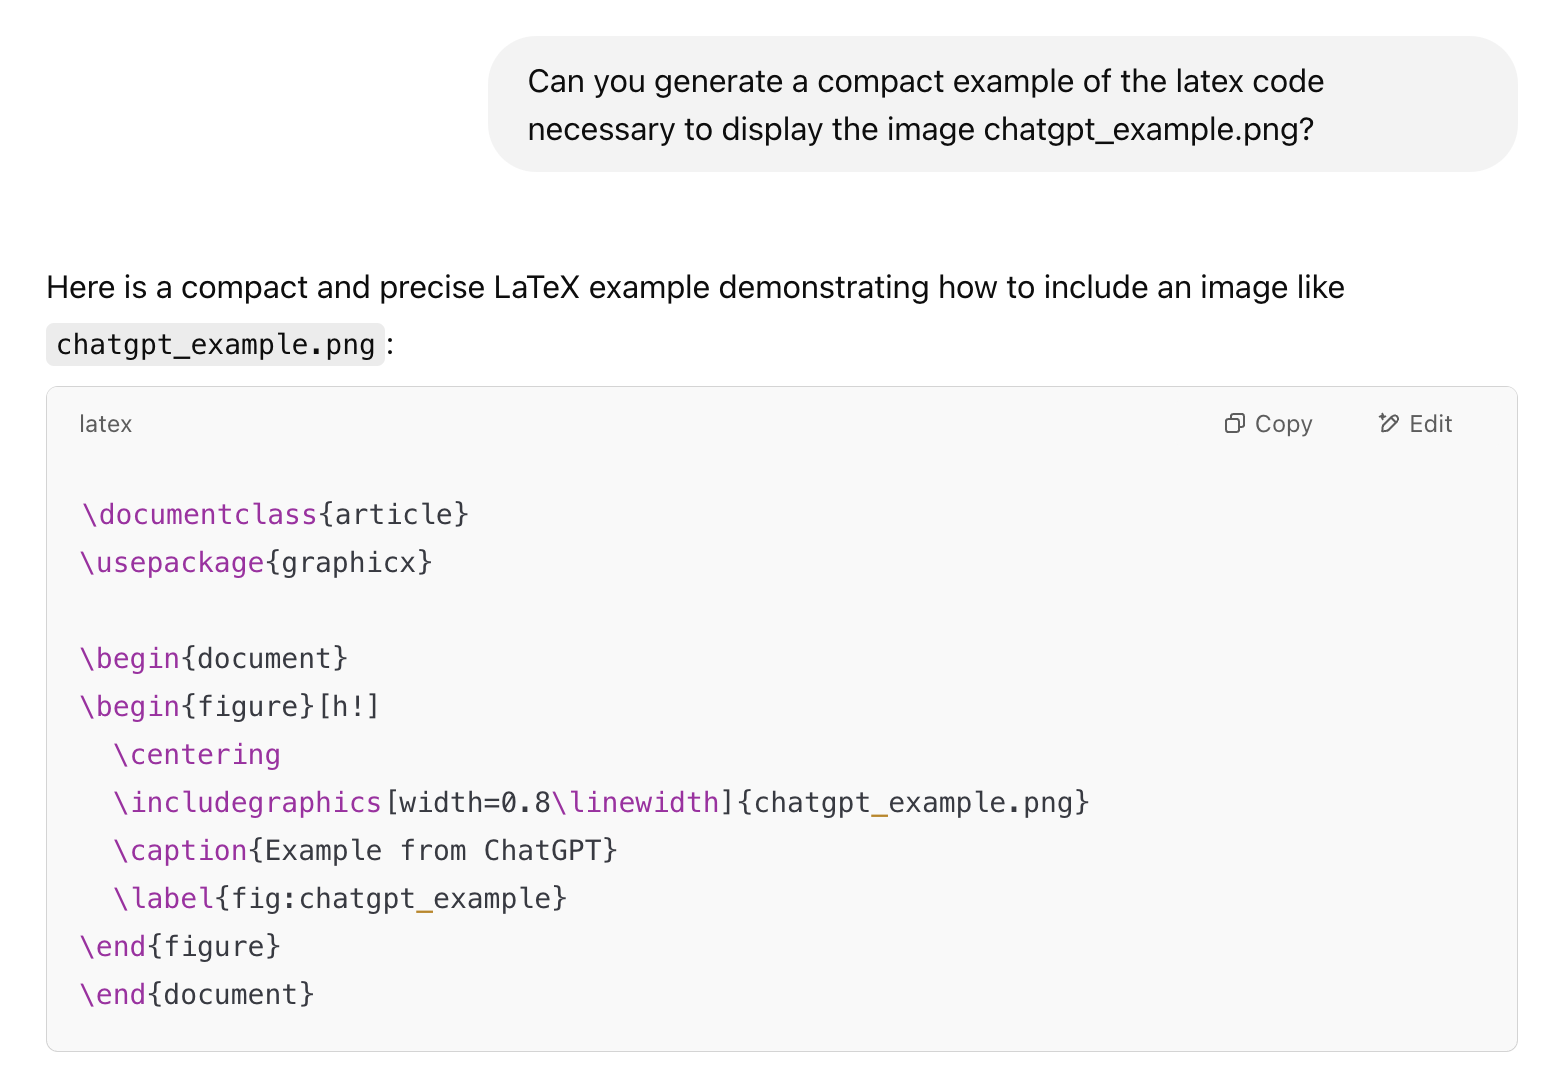
\includegraphics[width=9.5cm]{data/chatgpt_example.png}
				};
			}

			\only<2>{
				\node[font=\scriptsize] at (0, 0) {
					\url{https://chatgpt.com/c/67e95f86-538c-8013-a01d-4e057aa2a56d}
				};
			}

			\only<3>{
				\node[font=\scriptsize] at (0, 0) {
					\url{https://uio.instructure.com/courses/54846/assignments/127687}
				};
			}
			\only<4>{
				\node[font=\scriptsize] at (0, 0) {
					\url{https://uio.instructure.com/courses/54846/assignments/128391}
				};
			}
		\end{tikzpicture}
	\end{frame}
	\begin{frame}{Generativ AI i moderne programmering}
		\begin{tikzpicture}
			\node[] at (-5.25, -3.5) {};
			\node[] at (5.25, 3.5) {};

			\only<1>{
				\node[inner sep=0pt, draw=black] (cursor) at (0, 1) {
					
\includegraphics[width=11cm]{data/cursor.png}
				};
				\node[anchor=north, inner sep=8pt] at (cursor.south) {
					\url{https://www.cursor.com/}
				};
			}
			\visible<2-3>{
				\node[font=\tiny, anchor=south, text width=10.5cm, align=flush center] at (0, -3.85) {Kalliamvakou, E. (2022). \textit{Research: quantifying GitHub Copilot’s impact on developer productivity and happiness}. The GitHub Blog};
			}
			\only<2>{
				\node[inner sep=0pt, draw=black] at (0, 0) {
					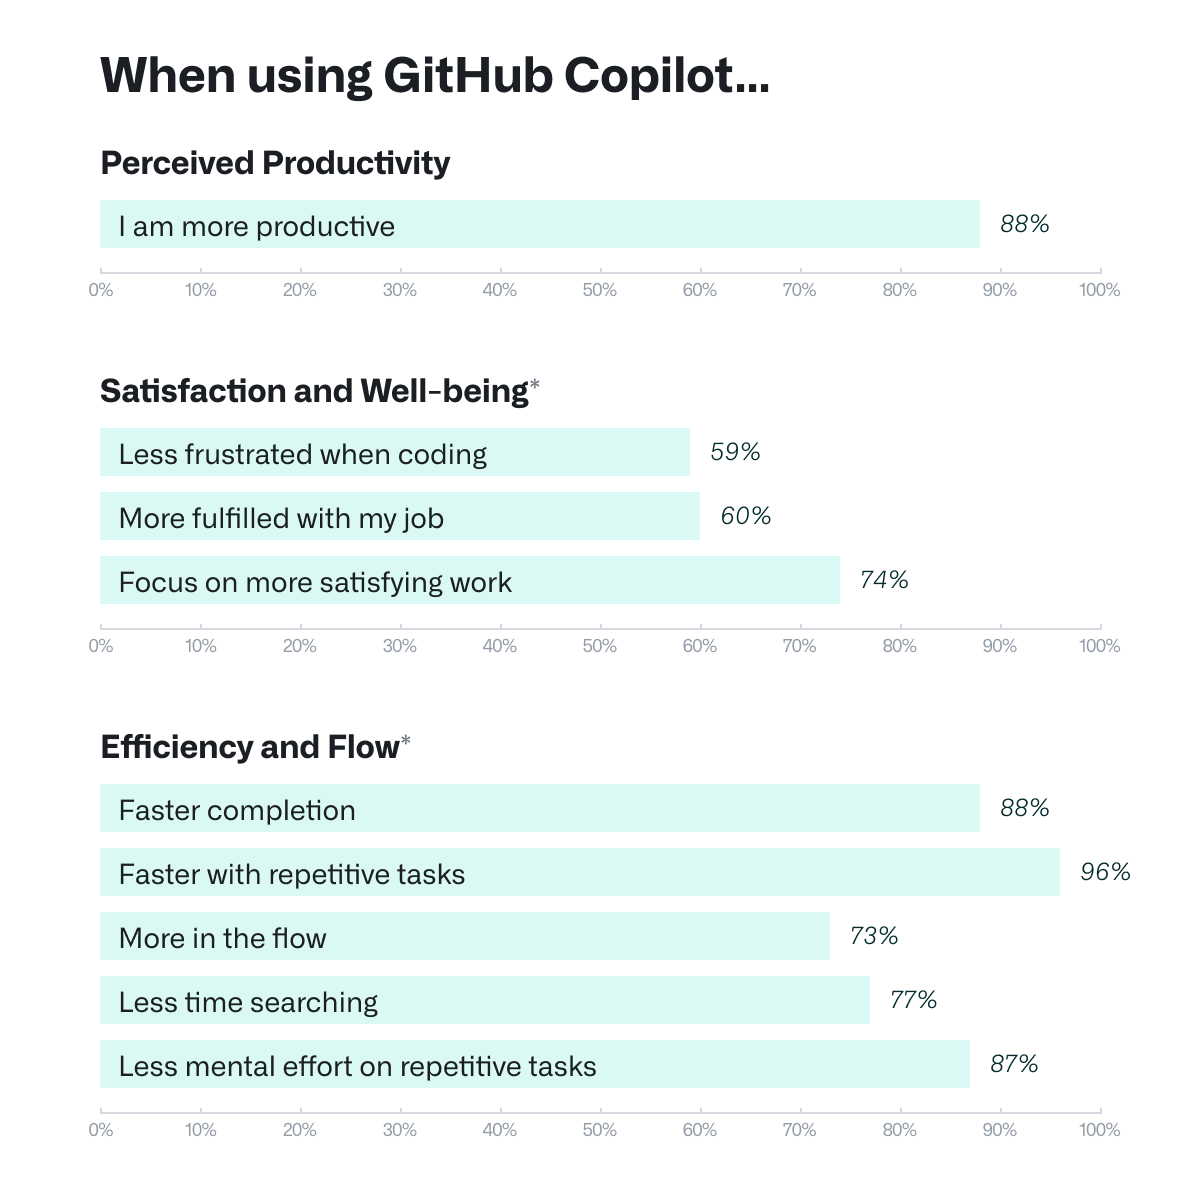
\includegraphics[width=5.5cm]{data/copilot1.png}
				};
			}
			\only<3>{
				\node[inner sep=0pt, draw=black] at (0, 0) {
					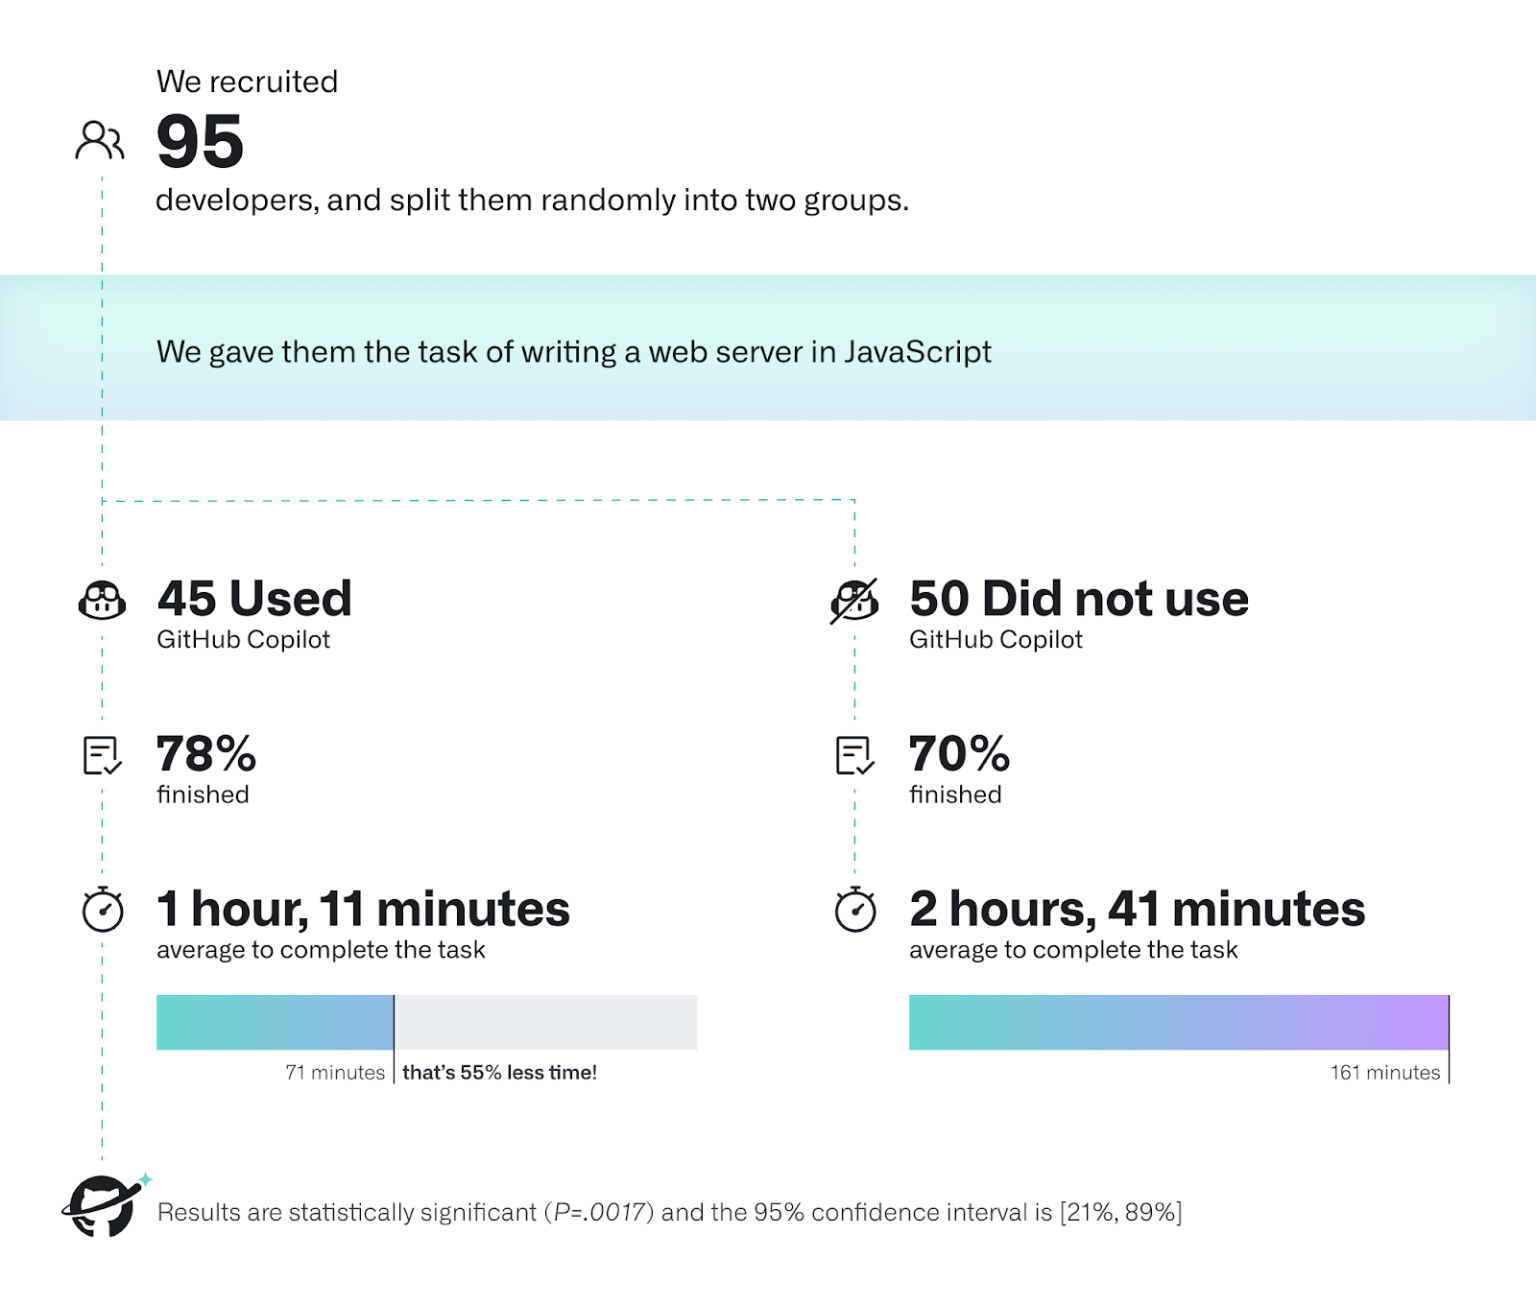
\includegraphics[width=6.5cm]{data/copilot2.png}
				};
			}
		\end{tikzpicture}
	\end{frame}

	\begin{frame}{Generativ AI i PSY9511}
		\begin{tikzpicture}
			\node[] at (-5.25, -3.5) {};
			\node[] at (5.25, 3.5) {};

			\only<1>{
				\node[inner sep=0pt, draw=black] at (0, 0) {
					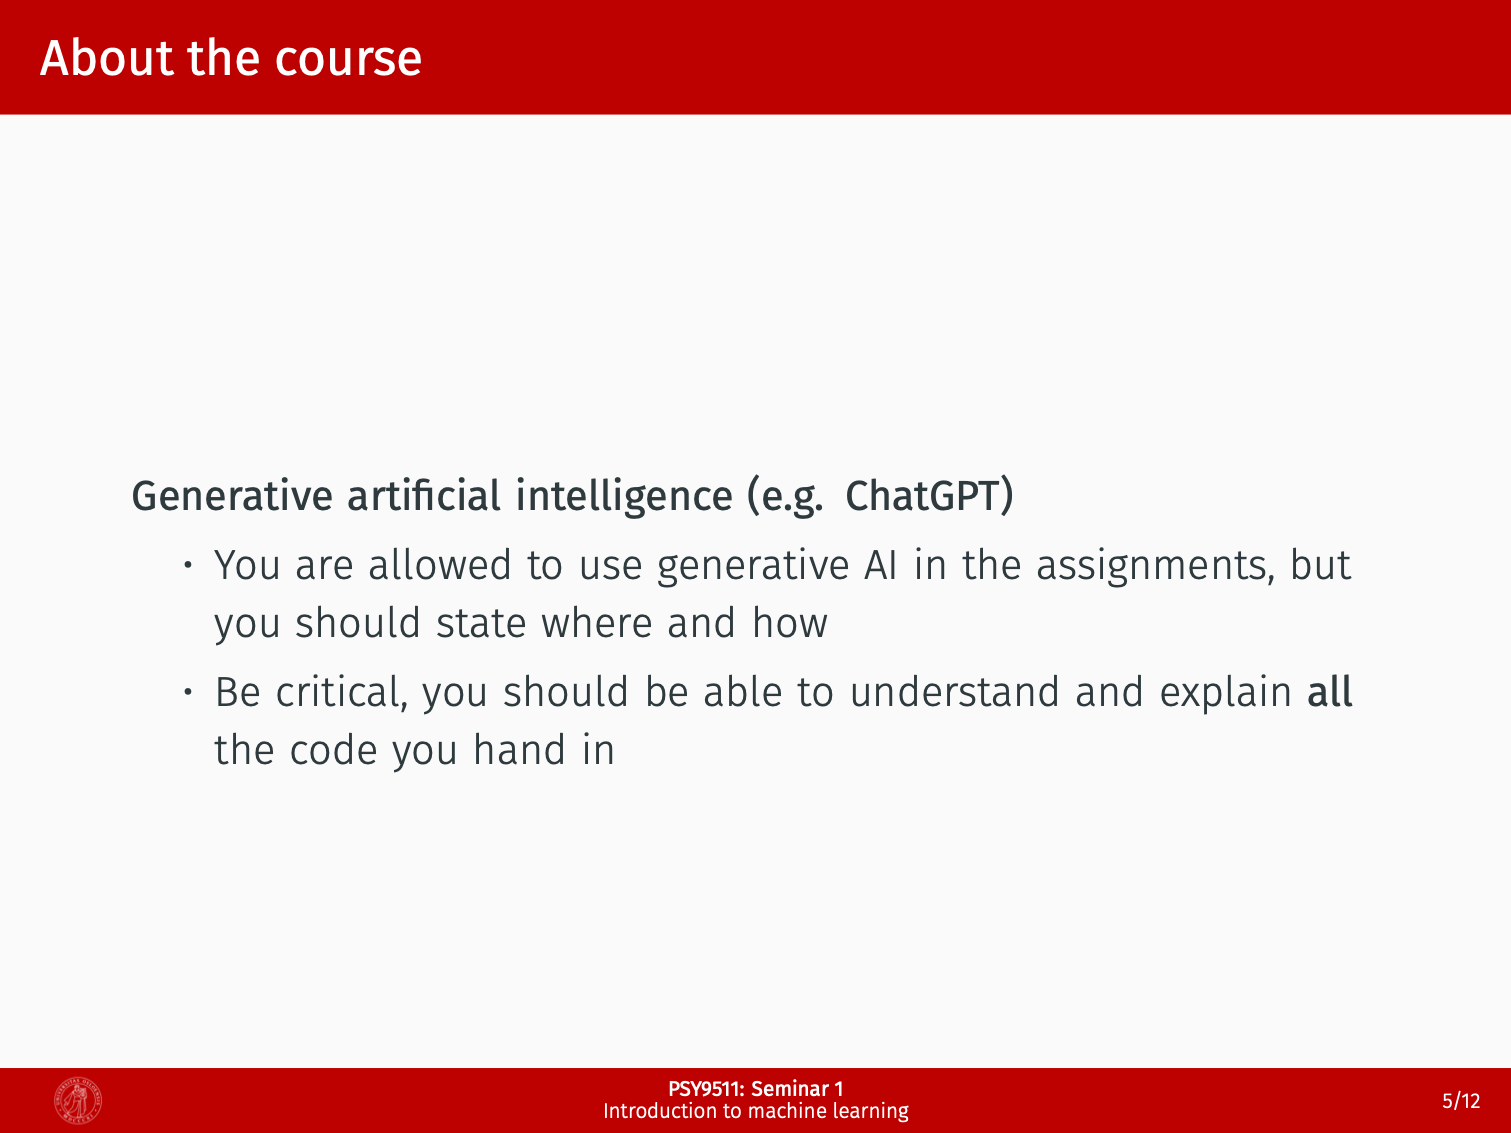
\includegraphics[width=8cm]{data/intro.png}
				};
			}
		\end{tikzpicture}
	\end{frame}
\end{document}
